% ======================================================================
%  From Audio to Beatmap -- the signal-processing pipeline
%  Build:  tectonic main.tex        (or: xelatex/pdflatex main.tex)
%  Data:   python make_data.py ../data/raw/bad_apple.mp3 --window 40 46
%          (every plot in this deck is read from data/, computed by the
%           generator's own functions)
% ======================================================================
\documentclass[aspectratio=169,11pt]{beamer}

\usepackage{amsmath,amssymb}
\usepackage{booktabs}
\usepackage{fancyvrb}
\usepackage{tikz}
\usepackage{pgfplots}
\pgfplotsset{compat=1.18}
\usetikzlibrary{arrows.meta,positioning,calc,shapes.geometric,shapes.misc,
                fit,backgrounds,decorations.pathreplacing,matrix}
\usepgfplotslibrary{fillbetween}

\input{data/stats.tex}

% ---------------------------------------------------------------- colours
\definecolor{void}{HTML}{1E1433}
\definecolor{ink}{HTML}{2B2540}
\definecolor{magenta}{HTML}{E0287D}
\definecolor{teal}{HTML}{0E9DB3}
\definecolor{amber}{HTML}{E89A1C}
\definecolor{mint}{HTML}{1FA868}
\definecolor{violet}{HTML}{8A3FE0}
\definecolor{paper}{HTML}{FBF9FE}
\definecolor{muted}{HTML}{8B84A0}

% ---------------------------------------------------------------- theme
\setbeamercolor{background canvas}{bg=paper}
\setbeamercolor{normal text}{fg=ink}
\setbeamercolor{frametitle}{fg=white,bg=void}
\setbeamercolor{title}{fg=white}
\setbeamercolor{subtitle}{fg=white!80!magenta}
\setbeamercolor{structure}{fg=magenta}
\setbeamercolor{alerted text}{fg=magenta}
\setbeamercolor{block title}{fg=white,bg=void}
\setbeamercolor{block body}{bg=void!6}
\setbeamerfont{frametitle}{series=\bfseries,size=\large}
\setbeamertemplate{navigation symbols}{}
\setbeamertemplate{itemize item}{\color{magenta}$\blacktriangleright$}
\setbeamertemplate{itemize subitem}{\color{teal}--}
\setbeamertemplate{frametitle}{%
  \nointerlineskip
  \begin{beamercolorbox}[wd=\paperwidth,ht=2.4ex,dp=1.1ex,leftskip=1.2em]{frametitle}
    \usebeamerfont{frametitle}\insertframetitle
    \hfill{\normalsize\normalfont\color{white!60!void}\insertsectionhead\hspace*{1.2em}}
  \end{beamercolorbox}%
  \vspace{-0.2ex}%
  
\begin{tikzpicture}[overlay]\fill[magenta] (0,0) rectangle (\paperwidth,0.06);\end{tikzpicture}%
}
\setbeamertemplate{footline}{%
  \hfill{\scriptsize\color{muted}\insertframenumber\hspace*{1.2em}}\vspace*{0.8ex}}

% ---------------------------------------------------------------- tikz
% overlay-aware styles: `visible on=<2->`, `alt=<3>{a}{b}`
\tikzset{
  invisible/.style={opacity=0,text opacity=0},
  visible on/.style={alt={#1{}{invisible}}},
  alt/.code args={<#1>#2#3}{\alt<#1>{\pgfkeysalso{#2}}{\pgfkeysalso{#3}}},
  stage/.style={draw=void!70,rounded corners=4pt,fill=white,minimum width=2.45cm,
                minimum height=1.05cm,align=center,font=\footnotesize\bfseries,line width=0.8pt},
  hot/.style={fill=magenta!14,draw=magenta,line width=1.6pt},
  cold/.style={fill=void!4,draw=void!25,text=muted},
  flow/.style={-{Stealth[length=2.2mm]},line width=0.9pt,color=void!65},
  hotflow/.style={-{Stealth[length=2.6mm]},line width=1.6pt,color=magenta},
  note/.style={font=\scriptsize,text=muted,align=center},
  data/.style={font=\scriptsize\ttfamily,fill=teal!10,draw=teal!60,rounded corners=2pt,
               inner sep=2.5pt,align=center},
  decision/.style={diamond,aspect=2.2,draw=void!70,fill=white,align=center,
                   font=\scriptsize\bfseries,inner sep=1pt,line width=0.8pt},
  outcome/.style={rounded corners=3pt,draw=#1,fill=#1!15,font=\scriptsize\bfseries,
                  minimum width=1.9cm,minimum height=0.6cm,line width=1pt},
  pfpath/.style={dashed,line width=0.7pt,color=void!55},
  pfcursor/.style={pfpath,shorten <=0.5cm,shorten >=0.5cm},
  pfbody/.style={color=teal!70!black,line cap=round,line join=round},
  pfbodyedge/.style={color=teal!18,line cap=round,line join=round},
  pfcircle/.style={circle,draw=magenta,line width=1.3pt,fill=white,
                   font=\scriptsize\bfseries,inner sep=0pt},
}
\pgfplotsset{
  every axis/.append style={font=\scriptsize,axis line style={void!50},tick style={void!50},
                            label style={font=\scriptsize}},
  dspaxis/.style={width=\linewidth,height=4.2cm,xmin=\statWinStart,xmax=\statWinEnd,
                  axis lines=left,enlarge y limits={upper,value=0.05},
                  xlabel={time (s)}},
}

% the pipeline strip shown at the top of each section: #1 = active step
\newcommand{\roadmap}[1]{%
  \begin{center}\begin{tikzpicture}[x=2.0cm]
    \foreach \i/\t in {1/STFT,2/Onsets,3/Tempo,4/Objects,5/Difficulty,6/Export,7/Analysis}{
      \ifnum\i=#1\relax
        \node[stage,hot,minimum width=1.62cm,minimum height=0.66cm,font=\scriptsize\bfseries] (r\i) at (\i,0) {\t};
      \else
        \node[stage,cold,minimum width=1.62cm,minimum height=0.66cm,font=\scriptsize] (r\i) at (\i,0) {\t};
      \fi
    }
    \foreach \i [evaluate=\i as \j using int(\i+1)] in {1,...,6}{\draw[flow,void!30] (r\i) -- (r\j);}
  \end{tikzpicture}\end{center}}

\newcommand{\sectionframe}[3]{% #1 step number, #2 title, #3 one-line question
  \begin{frame}[plain]
    \vfill\roadmap{#1}\vspace{1.2em}
    \begin{center}
      {\color{magenta}\large\bfseries Step #1}\\[0.3em]
      {\color{void}\huge\bfseries #2}\\[0.8em]
      {\color{muted}\large #3}
    \end{center}\vfill
  \end{frame}}

\title{From Audio to Beatmap}
\subtitle{A signal-processing pipeline that turns any song into a playable osu!\ map}
\date{}

% ======================================================================
\begin{document}

% ---------------------------------------------------------------- title
\begin{frame}[plain]
  \begin{tikzpicture}[remember picture,overlay]
    \fill[void] (current page.south west) rectangle (current page.north east);
    % a stylised flux curve along the bottom
    \begin{scope}[shift={($(current page.south west)+(0,1.1)$)}]
      \draw[magenta,line width=1.2pt]
        plot[smooth,domain=0:16,samples=220]
          (\x,{0.35*sin(\x*300)*sin(\x*300)*sin(\x*300)*sin(\x*300)*sin(\x*300)*sin(\x*300)*(1+0.6*sin(\x*47))+0.05});
      \draw[teal,line width=0.8pt,dashed] (0,0.32) -- (16,0.32);
    \end{scope}
    \node[anchor=west,text width=12cm] at ($(current page.west)+(1.2,0.7)$) {%
      {\color{white}\fontsize{30}{34}\selectfont\bfseries From Audio to Beatmap}\\[0.5em]
      {\color{white!75!magenta}\large A signal-processing pipeline that turns any song\\ into a playable five-difficulty osu!\ beatmap set}};
    \node[anchor=west,text=white!55!void,font=\small] at ($(current page.west)+(1.2,-1.6)$)
      {audio file $\;\longrightarrow\;$ STFT $\;\to\;$ spectral flux $\;\to\;$ autocorrelation $\;\to\;$ \texttt{.osz}};
  \end{tikzpicture}
\end{frame}

% ---------------------------------------------------------------- problem
\begin{frame}{The problem}
  \begin{columns}[T]
    \begin{column}{0.47\textwidth}
      A \textbf{beatmap} is a timed list of things to click:
      \begin{itemize}
        \item \textbf{circles} -- tap on a beat
        \item \textbf{sliders} -- hold and follow a path
        \item \textbf{spinners} -- spin for a sustained passage
      \end{itemize}
      \medskip
      Each needs a \alert{time} (ms), a \alert{position} on a
      $512\times384$ playfield, and a \alert{type}.\\[0.8em]
      Human mappers do this by ear, for hours per song.\\[0.8em]
      \uncover<2->{\textbf{Goal:} derive all three from the audio signal alone,
      and write a file the real game imports.}
    \end{column}
    \begin{column}{0.5\textwidth}
      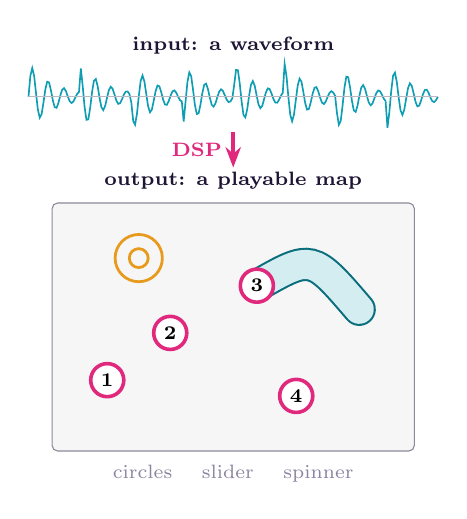
\begin{tikzpicture}[x=1cm,y=1cm]
        % waveform
        \node[font=\scriptsize\bfseries,text=void] at (2.6,3.55) {input: a waveform};
        \draw[teal,line width=0.6pt] plot[domain=0:5.2,samples=220]
          (\x,{2.9+0.42*sin(\x*1800)*exp(-3*mod(\x,0.65))});
        \draw[void!30] (0,2.9) -- (5.2,2.9);
        % arrow
        \draw<2->[hotflow] (2.6,2.45) -- (2.6,2.0) node[midway,left,font=\scriptsize\bfseries,text=magenta] {DSP};
        % playfield
        \begin{scope}[visible on=<2->]
          \draw[void!50,fill=void!4,rounded corners=2pt] (0.3,-1.6) rectangle (4.9,1.55);
          \node[font=\scriptsize\bfseries,text=void,anchor=south] at (2.6,1.6) {output: a playable map};
          \draw[teal!70!black,line width=12pt,line cap=round] (2.9,0.5) .. controls (3.6,0.9) .. (4.2,0.2);
          \draw[teal!18,line width=10.5pt,line cap=round] (2.9,0.5) .. controls (3.6,0.9) .. (4.2,0.2);
          \foreach \p/\n in {{(1.0,-0.7)}/1,{(1.8,-0.1)}/2,{(2.9,0.5)}/3,{(3.4,-0.9)}/4}
            \node[pfcircle,minimum size=0.42cm] at \p {\n};
          \draw[amber,line width=1pt] (1.4,0.85) circle (0.3) (1.4,0.85) circle (0.12);
          \node[note,anchor=north] at (2.6,-1.65) {circles \quad slider \quad spinner};
        \end{scope}
      \end{tikzpicture}
    \end{column}
  \end{columns}
\end{frame}

% ---------------------------------------------------------------- overview (animated)
\begin{frame}{The pipeline at a glance}
  \centering
  \begin{tikzpicture}[x=1cm,y=1cm]
    \node[data] (in) at (-0.2,2.2) {song.mp3};
    \node[stage,alt=<2>{hot}{}] (s1) at (2.4,2.2) {1\\Load \& STFT};
    \node[stage,alt=<3>{hot}{}] (s2) at (5.3,2.2) {2\\Onset detection};
    \node[stage,alt=<4>{hot}{}] (s3) at (8.2,2.2) {3\\Tempo \& beat grid};
    \node[stage,alt=<5>{hot}{}] (s4) at (11.1,2.2) {4\\Objects \&\\placement};
    \node[stage,alt=<6>{hot}{}] (s5) at (11.1,0.0) {5\\Difficulty\\ $\times5$ tiers};
    \node[stage,alt=<7>{hot}{}] (s6) at (8.2,0.0) {6\\\texttt{.osu} / \texttt{.osz}};
    \node[stage,alt=<8>{hot}{}] (s7) at (5.3,0.0) {7\\Analysis export};
    \node[data] (out) at (2.4,0.0) {Artist - Song.osz\\+ analysis.json};

    \draw[flow,alt=<2>{hotflow}{}] (in) -- (s1);
    \draw[flow,alt=<3>{hotflow}{}] (s1) -- (s2);
    \draw[flow,alt=<4>{hotflow}{}] (s2) -- (s3);
    \draw[flow,alt=<5>{hotflow}{}] (s3) -- (s4);
    \draw[flow,alt=<6>{hotflow}{}] (s4) -- (s5);
    \draw[flow,alt=<7>{hotflow}{}] (s5) -- (s6);
    \draw[flow,alt=<8>{hotflow}{}] (s6) -- (s7);
    \draw[flow] (s7) -- (out);
    % the onsets skip ahead to Step 4 as well
    \draw[flow,dashed,alt=<5>{hotflow}{}] (s2.north) to[out=35,in=145] node[above,note] {onsets} (s4.north);

    \begin{scope}[on background layer]
      \node[fit=(s1)(s2)(s3),fill=teal!7,rounded corners=6pt,inner sep=7pt,
            label={[note,text=teal!70!black,anchor=north west]south west:signal analysis}] {};
      \node[fit=(s4)(s5),fill=magenta!6,rounded corners=6pt,inner sep=7pt,
            label={[note,text=magenta,anchor=north]south:musical decisions}] {};
    \end{scope}

    \node[note,text width=12.5cm,anchor=north] at (5.6,-1.2) {%
      \only<1>{One command: \texttt{python src/main.py song.mp3} $\rightarrow$ five difficulties, Easy to Expert.}%
      \only<2>{Decode, resample to \statSampleRate\ Hz mono, then a short-time Fourier transform on a mel frequency scale.}%
      \only<3>{Spectral flux measures \emph{energy appearing}; an adaptive threshold picks the note attacks.}%
      \only<4>{Autocorrelation of the flux finds the beat period; a pulse-train search finds its phase.}%
      \only<5>{Onsets snapped to the grid become circles, sliders or spinners, placed the way a human mapper would.}%
      \only<6>{The same analysis is re-read with five parameter sets -- sensitivity, grid, spacing, circle size.}%
      \only<7>{Rendered as \texttt{osu file format v14} and zipped into an \texttt{.osz} the game imports.}%
      \only<8>{What the DSP saw (onsets, grid, spectrogram) is saved for the app's visualisation.}};
  \end{tikzpicture}
\end{frame}

\begin{frame}{Running example}
  \begin{columns}[c]
    \begin{column}{0.52\textwidth}
      Every plot in this talk is \textbf{real output} of the generator,
      computed by its own functions on one song:
      \begin{itemize}
        \item \textbf{\SongFile} -- \statDuration\,s, decoded at \statSampleRate\,Hz
        \item zoomed plots show \statWinStart--\statWinEnd\,s
        \item per-tier numbers use the \textbf{\statTier} preset unless stated
      \end{itemize}
      \medskip
      {\color{muted}\small The data is regenerated by \texttt{presentation/make\_data.py},
      so the figures cannot drift from the code.}
    \end{column}
    \begin{column}{0.45\textwidth}
      \begin{tikzpicture}
        \begin{axis}[width=\linewidth,height=4.2cm,axis lines=left,xmin=\statWinStart,xmax=\statWinEnd,
                     ymin=-1.05,ymax=1.05,xlabel={time (s)},ylabel={amplitude}]
          \addplot[name path=lo,draw=none] table[col sep=comma,x=t,y=lo]{data/wave.csv};
          \addplot[name path=hi,draw=none] table[col sep=comma,x=t,y=hi]{data/wave.csv};
          \addplot[teal!70] fill between[of=lo and hi];
        \end{axis}
      \end{tikzpicture}
      \par\centering\color{muted}\scriptsize peak-normalised waveform, \statWinStart--\statWinEnd\,s\par
    \end{column}
  \end{columns}
\end{frame}

% ======================================================================
\sectionframe{1}{Loading \& time-frequency analysis}{What does the song contain, and when?}
\section{1 \;Load \& STFT}

\begin{frame}{Loading: a consistent signal to analyse}
  \centering
  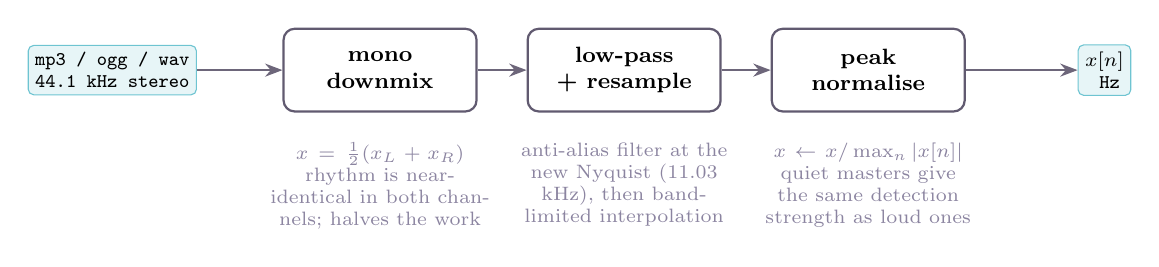
\begin{tikzpicture}[x=1cm,y=1cm]
    \node[data] (f) at (0,0) {mp3 / ogg / wav\\44.1 kHz stereo};
    \node[stage,visible on=<2->] (m) at (3.4,0) {mono\\downmix};
    \node[stage,visible on=<3->] (r) at (6.5,0) {low-pass\\+ resample};
    \node[stage,visible on=<4->] (n) at (9.6,0) {peak\\normalise};
    \node[data,visible on=<4->] (o) at (12.6,0) {$x[n]$\\\statSampleRate\ Hz};
    \draw[flow,visible on=<2->] (f) -- (m);
    \draw[flow,visible on=<3->] (m) -- (r);
    \draw[flow,visible on=<4->] (r) -- (n);
    \draw[flow,visible on=<4->] (n) -- (o);
    \node[note,text width=2.8cm,anchor=north,visible on=<2->] at (3.4,-0.8)
      {$x=\tfrac12(x_L+x_R)$\\rhythm is near-identical in both channels; halves the work};
    \node[note,text width=2.9cm,anchor=north,visible on=<3->] at (6.5,-0.8)
      {anti-alias filter at the new Nyquist (11.03 kHz), then band-limited interpolation};
    \node[note,text width=2.8cm,anchor=north,visible on=<4->] at (9.6,-0.8)
      {$x \leftarrow x/\max_n|x[n]|$\\quiet masters give the same detection strength as loud ones};
  \end{tikzpicture}
  \vspace{1.2em}

  \uncover<5->{\begin{block}{Why 22.05 kHz is enough}
    Onsets and beats live in how energy \emph{changes over time}; content above
    11 kHz (cymbal shimmer) adds almost nothing, and half the samples halves every later cost.
  \end{block}}
\end{frame}

\begin{frame}{The short-time Fourier transform}
  \begin{columns}[T]
    \begin{column}{0.55\textwidth}
      \begin{tikzpicture}
        \begin{axis}[width=\linewidth,height=4.6cm,axis lines=left,xmin=0,xmax=300,ymin=-1.05,ymax=1.35,
                     xlabel={time (ms)},ytick=\empty,clip=false]
          \addplot[teal!60,line width=0.4pt] table[col sep=comma,x=ms,y=y]{data/wave_zoom.csv};
          \foreach \m/\c in {0/magenta,1/violet,2/amber,3/mint}{
            \edef\temp{\noexpand\only<\the\numexpr\m+1\relax->{
              \noexpand\addplot[\c,line width=1pt,domain=\m*23.22:\m*23.22+92.88,samples=60]
                {1.2*sin(deg(pi*(x-\m*23.22)/92.88))^2};
              \noexpand\draw[\c,fill=\c,fill opacity=0.07,draw opacity=0.6]
                (axis cs:\m*23.22,-1.05) rectangle (axis cs:\m*23.22+92.88,1.25);}}
            \temp
          }
          \only<2->{\draw[{Stealth}-{Stealth},void] (axis cs:0,1.3) -- node[above,font=\scriptsize] {hop $H$} (axis cs:23.22,1.3);}
        \end{axis}
      \end{tikzpicture}
      \par\centering\color{muted}\scriptsize the first 300\,ms, a Hann window every hop\par
    \end{column}
    \begin{column}{0.43\textwidth}
      Slide a window $w$ along the signal; each position gives one spectrum:
      \[
        X[m,k]=\sum_{n=0}^{N-1} x[n+mH]\,w[n]\,e^{-j2\pi kn/N}
      \]
      \vspace{-0.6em}
      \begin{center}\small
      \begin{tabular}{@{}ll@{}}
        \toprule
        window $N$ & \statNFFT\ samples = \statWinMs\,ms\\
        hop $H$ & \statHop\ samples = \statHopMs\,ms\\
        frame rate & \statFrameRate\ spectra / s\\
        bin width & $f_s/N$ = \statBinHz\,Hz\\
        \bottomrule
      \end{tabular}
      \end{center}
      \uncover<5->{\small\alert{Trade-off:} a longer window resolves pitch better but smears
      \emph{when} a hit happens. $23$\,ms steps are finer than any hit a player can react to.}
    \end{column}
  \end{columns}
\end{frame}

\begin{frame}{The mel scale}
  \begin{columns}[c]
    \begin{column}{0.55\textwidth}
      \begin{tikzpicture}
        \begin{axis}[width=\linewidth,height=4.6cm,axis lines=left,xmin=0,xmax=2200,ymin=0,ymax=1.1,
                     xlabel={frequency (Hz)},ylabel={filter weight},cycle list={
                     {magenta},{teal},{amber},{violet},{mint},{magenta!60},{teal!60},{amber!60},
                     {violet!60},{mint!60},{magenta!40},{teal!40}}]
          \foreach \i in {0,...,11}{\addplot+[no marks,line width=0.9pt] table[col sep=comma,x=f,y=m\i]{data/melfb.csv};}
        \end{axis}
      \end{tikzpicture}
      \par\centering\color{muted}\scriptsize lowest filters of a mel filterbank (drawn with 24 bands)\par
    \end{column}
    \begin{column}{0.43\textwidth}
      Pool the \statNFFT/2+1 linear bins into \textbf{128 triangular bands}
      spaced evenly in mel:
      \[ \mathrm{mel}(f)=2595\,\log_{10}\!\left(1+\frac{f}{700}\right) \]
      \begin{itemize}
        \item narrow bands low (kick, bass), wide bands high
        \item matches pitch perception, and where rhythm lives
        \item power $\rightarrow$ dB for display: $10\log_{10}P$
      \end{itemize}
    \end{column}
  \end{columns}
\end{frame}

\begin{frame}{The result: a mel spectrogram}
  \centering
  \begin{tikzpicture}
    % one picture, both axes anchored at the same x, so time lines up exactly
    \begin{axis}[at={(0,3.95cm)},anchor=south west,width=0.86\linewidth,height=1.4cm,scale only axis,
                 axis lines=left,xmin=\statWinStart,xmax=\statWinEnd,ymin=-1.05,ymax=1.05,
                 xticklabels=\empty,ylabel={$x[n]$},ytick=\empty]
      \addplot[name path=lo,draw=none] table[col sep=comma,x=t,y=lo]{data/wave.csv};
      \addplot[name path=hi,draw=none] table[col sep=comma,x=t,y=hi]{data/wave.csv};
      \addplot[teal!70] fill between[of=lo and hi];
    \end{axis}
    \begin{axis}[at={(0,0)},anchor=south west,width=0.86\linewidth,height=3.4cm,scale only axis,
                 axis lines=left,xmin=\statWinStart,xmax=\statWinEnd,ymin=0,ymax=128,
                 xlabel={time (s)},ylabel={mel band},enlargelimits=false,ytick={0,64,128}]
      \addplot graphics[xmin=\statWinStart,xmax=\statWinEnd,ymin=0,ymax=128]{data/melspec.png};
      \only<2->{\draw[white,dashed] (axis cs:\statFluxOnsetTime,0) -- (axis cs:\statFluxOnsetTime,128);}
    \end{axis}
  \end{tikzpicture}
  \par\raggedright
  \vspace{-0.5em}
  {\small\color{muted}\statNFrames\ frames $\times$ 128 bands for the whole song.
  \uncover<2->{\color{ink}Vertical streaks = broadband attacks: \alert{that is what we want to detect}.}}
\end{frame}

% ======================================================================
\sectionframe{2}{Onset detection}{When does a new sound start?}
\section{2 \;Onsets}

\begin{frame}{Spectral flux: measuring energy that \emph{appears}}
  \begin{columns}[T]
    \begin{column}{0.56\textwidth}
      \begin{tikzpicture}
        \pgfplotsset{fluxbars/.style={width=\linewidth,height=4.9cm,axis lines=left,ybar,bar width=4pt,
                     xmin=0.3,xmax=16.7,xlabel={mel band group (low $\rightarrow$ high)},
                     xtick={1,4,8,12,16},
                     legend style={font=\tiny,at={(0.02,1)},anchor=north west,draw=none,fill=none},
                     legend cell align=left}}
        \only<1-2>{%
        \begin{axis}[fluxbars,ymin=0,ymax=1.1,ylabel={level (dB, scaled)}]
          \addplot[fill=void!35,draw=none,bar shift=-2pt] table[col sep=comma,x=band,y=prev]{data/fluxbars.csv};
          \addlegendentry{frame $m-1$}
          \only<2>{\addplot[fill=magenta!70,draw=none,bar shift=2pt] table[col sep=comma,x=band,y=cur]{data/fluxbars.csv};
                   \addlegendentry{frame $m$ (onset)}}
        \end{axis}}%
        \only<3->{%
        \begin{axis}[fluxbars,ymin=-0.05,ymax=0.13,ylabel={change}]
          \only<3>{\addplot[fill=teal,draw=none] table[col sep=comma,x=band,y=diff]{data/fluxbars.csv};
                   \addlegendentry{difference}}
          \only<4->{\addplot[fill=magenta,draw=none] table[col sep=comma,x=band,y=rect]{data/fluxbars.csv};
                    \addlegendentry{rectified $\max(0,\cdot)$}}
          \draw[void!40] (axis cs:0.3,0) -- (axis cs:16.7,0);
        \end{axis}}
      \end{tikzpicture}
      \par\centering\color{muted}\scriptsize the onset at \statFluxOnsetTime\,s: \statFluxRises\ of 16 groups get louder at once\par
    \end{column}
    \begin{column}{0.42\textwidth}
      \only<1>{Compare each spectrum with the one before it.}
      \only<2>{At an attack, energy jumps up across many bands at once.}
      \only<3>{Subtract frame by frame. Negative values are notes \emph{decaying} -- not new events.}
      \only<4->{Keep only increases (half-wave rectify), then take the norm across bands:}
      \uncover<4->{
      \[ \Delta P[m,k]=P[m,k]-P[m-1,k] \]
      \[ \mathrm{SF}[m]=\sqrt{\textstyle\sum_{k}\max\big(0,\Delta P[m,k]\big)^{2}} \]}
      \uncover<5->{\small
      \begin{itemize}
        \item computed on \textbf{linear power} -- differences of dB values over-weight quiet noise
        \item one number per frame: \statFrameRate\ values / s
        \item then min--max normalised to $[0,1]$
      \end{itemize}}
    \end{column}
  \end{columns}
\end{frame}

\begin{frame}{Adaptive threshold}
  \begin{tikzpicture}
    \begin{axis}[dspaxis,height=4.9cm,ymin=0,ymax=1.05,ylabel={normalised flux},
                 legend style={font=\tiny,at={(1,1.02)},anchor=south east,draw=none,fill=none,legend columns=4}]
      \addplot[void!55,line width=0.6pt] table[col sep=comma,x=t,y=flux]{data/flux.csv};
      \addlegendentry{$\mathrm{SF}[m]$}
      \only<2->{\addplot[teal,line width=1.1pt] table[col sep=comma,x=t,y=median]{data/flux.csv};
                \addlegendentry{moving median}}
      \only<3->{\addplot[magenta,line width=1.3pt] table[col sep=comma,x=t,y=thr]{data/flux.csv};
                \addlegendentry{threshold $T[m]$}}
      \only<4->{\addplot[only marks,mark=*,mark size=1.8pt,amber] table[col sep=comma,x=t,y=s]{data/peaks.csv};
                \addlegendentry{picked onsets}}
    \end{axis}
  \end{tikzpicture}
  \vspace{-0.3em}
  \begin{columns}[T]
    \begin{column}{0.5\textwidth}
      \[ T[m]=\delta+\lambda\cdot\operatorname*{median}_{|i-m|\le w}\mathrm{SF}[i] \]
      \vspace{-1.2em}
      {\small $w=0.5$\,s, \ \statTier: $\lambda=\statMargin$, $\delta=\statDelta$}
    \end{column}
    \begin{column}{0.48\textwidth}\small
      \only<1-2>{\textbf{Median}, not mean: the spikes themselves don't drag the floor up. It
      tracks the local loudness of a quiet verse or a loud drop.}
      \only<3>{$\lambda$ scales with the floor; $\delta$ is a hard floor so near-silence never
      turns noise into onsets (found with a synthetic noise test).}
      \only<4->{\textbf{Peak picking}: a local maximum above $T[m]$, at least 50\,ms after the
      last kept one (else keep the stronger). \statOnsetsWindow\ onsets here,
      \statOnsetsTotal\ in the song.}
    \end{column}
  \end{columns}
\end{frame}

\begin{frame}{Band-limited flux: \emph{what kind} of onset}
  \begin{columns}[c]
    \begin{column}{0.6\textwidth}
      \begin{tikzpicture}
        \begin{axis}[dspaxis,height=5.2cm,ymin=0,ymax=3.3,ytick={0.5,1.6,2.7},
                     yticklabels={high,mid,low},ylabel={}]
          \addplot[violet,line width=0.6pt] table[col sep=comma,x=t,y expr=\thisrow{high}*0.95+0.05]{data/bands.csv};
          \addplot[teal,line width=0.6pt] table[col sep=comma,x=t,y expr=\thisrow{mid}*0.95+1.15]{data/bands.csv};
          \addplot[magenta,line width=0.6pt] table[col sep=comma,x=t,y expr=\thisrow{low}*0.95+2.25]{data/bands.csv};
          \only<2->{\addplot[ycomb,amber!80,line width=0.5pt,opacity=0.7] table[col sep=comma,x=t,y expr=3.3]{data/peaks.csv};}
        \end{axis}
      \end{tikzpicture}
    \end{column}
    \begin{column}{0.38\textwidth}
      The same flux, restricted to three bands:
      \begin{center}\small
      \begin{tabular}{@{}lll@{}}
        \toprule
        low & 20--200 Hz & kick, bass\\
        mid & 200--2000 Hz & snare, vocals\\
        high & 2--10 kHz & hats, cymbals\\
        \bottomrule
      \end{tabular}
      \end{center}
      \uncover<2->{Each onset records its \textbf{dominant band} and its \textbf{strength}.
      They cost nothing extra and travel with the onset as provenance, all the way to the
      exported analysis.}
    \end{column}
  \end{columns}
\end{frame}

% ======================================================================
\sectionframe{3}{Tempo \& beat grid}{How fast is the music, and where is beat one?}
\section{3 \;Tempo \& grid}

\begin{frame}{Autocorrelation reveals the period}
  \begin{columns}[T]
    \begin{column}{0.55\textwidth}
      \begin{tikzpicture}
        \begin{axis}[width=\linewidth,height=4.8cm,axis lines=left,xmin=0,xmax=2.5,ymin=-0.3,ymax=1.05,
                     xlabel={lag $\ell$ (s)},ylabel={$r[\ell]$}]
          \addplot[void!60,line width=0.8pt] table[col sep=comma,x=lag,y=acf]{data/acf_lag.csv};
          \only<2->{\foreach \k in {1,2,3,4,5}{
            \edef\temp{\noexpand\draw[magenta,dashed] (axis cs:{\k*\statBeatMs/1000},-0.3) -- (axis cs:{\k*\statBeatMs/1000},1.0);}\temp}
            \node[magenta,font=\scriptsize,anchor=south west] at (axis cs:{\statBeatMs/1000},0.72) {$\ell^\ast=\statBeatMs$\,ms};}
        \end{axis}
      \end{tikzpicture}
    \end{column}
    \begin{column}{0.43\textwidth}
      A beat is a \emph{repeating} ripple in the flux.
      Correlating the envelope with a shifted copy of itself:
      \[ r[\ell]=\frac{\sum_m \tilde e[m]\,\tilde e[m+\ell]}{\sum_m \tilde e[m]^2},\quad \tilde e=e-\bar e \]
      \uncover<2->{peaks at the beat period and all its multiples.}
      \uncover<3->{\small\medskip
      Computed with the \textbf{Wiener--Khinchin} theorem, $O(n\log n)$:
      \[ r=\mathcal{F}^{-1}\big\{|\mathcal{F}\{\tilde e\}|^2\big\} \]
      (zero-padded to avoid circular wrap-around).}
    \end{column}
  \end{columns}
\end{frame}

\begin{frame}{From lag to BPM, with a perceptual prior}
  \begin{columns}[T]
    \begin{column}{0.56\textwidth}
      \begin{tikzpicture}
        \begin{axis}[width=\linewidth,height=5cm,axis lines=left,xmin=50,xmax=210,ymin=0,ymax=1.05,
                     xlabel={tempo (BPM)},legend style={font=\tiny,at={(0.5,1.03)},anchor=south,draw=none,fill=none,legend columns=3},
                     legend cell align=left]
          \addplot[void!55,mark=*,mark size=1pt,line width=0.6pt] table[col sep=comma,x=bpm,y=acf]{data/acf.csv};
          \addlegendentry{$r$ at each lag}
          \only<2->{\addplot[teal,dashed,line width=1pt,domain=50:210,samples=100]{exp(-0.5*(ln(x/120)/ln(2))^2)};
                    \addlegendentry{prior $w(b)$}}
          \only<3->{\addplot[magenta,mark=*,mark size=1.2pt,line width=1.1pt] table[col sep=comma,x=bpm,y=weighted]{data/acf.csv};
                    \addlegendentry{$r\cdot w$}
                    \draw[magenta,dashed] (axis cs:\statRawBPM,0) -- (axis cs:\statRawBPM,1);}
        \end{axis}
      \end{tikzpicture}
    \end{column}
    \begin{column}{0.42\textwidth}\small
      Search lags for \textbf{50--210 BPM} only: \quad $b=\dfrac{60\,f_s}{H\,\ell}$\\[0.6em]
      \uncover<2->{A log-normal \textbf{tempo prior} centred on 120 BPM, where human tempo
      perception clusters (Parncutt 1994):
      \[ w(b)=\exp\!\Big(-\tfrac12\big(\log_2\tfrac{b}{120}\big)^2\Big) \]}
      \uncover<3->{The weighted peak, refined to sub-frame precision by a parabola through
      its neighbours:
      \[ \ell^\ast=i+\tfrac12\,\frac{r_{i-1}-r_{i+1}}{r_{i-1}-2r_i+r_{i+1}} \]
      $\Rightarrow$ \textbf{\statRawBPM\ BPM} (lag \statLagFrames\ frames).}
    \end{column}
  \end{columns}
\end{frame}

\begin{frame}{Octave correction}
  Autocorrelation peaks equally at $\tfrac12\times$, $1\times$ and $2\times$ the true tempo --
  the classic failure of tempo estimation. \\[0.4em]
  Re-score each candidate by \emph{how well a pulse train at that tempo lands on real onset energy}:
  \[ \text{score}(b)=\underbrace{\frac{\text{mean envelope on the beats}}{\text{mean envelope overall}}}_{\text{phase strength}}\times\;w(b) \]
  \begin{center}
  \begin{tikzpicture}
    \matrix[matrix of nodes,ampersand replacement=\&,nodes={minimum width=2.4cm,minimum height=0.62cm,font=\small,anchor=center},
            row 1/.style={nodes={font=\small\bfseries,text=void}},column sep=2pt,row sep=1pt] (t) {
      candidate \& tempo \& phase strength \& prior $w$ \& score \\
      $\tfrac12\times$ \& \statOctHalfBPM \& \statOctHalfPhase \& \statOctHalfPrior \& \statOctHalfScore \\
      $1\times$ \& \statOctOneBPM \& \statOctOnePhase \& \statOctOnePrior \& \statOctOneScore \\
      $2\times$ \& \statOctDoubleBPM \& \statOctDoublePhase \& \statOctDoublePrior \& \statOctDoubleScore \\
    };
    \draw[void!40] (t-1-1.south west) -- (t-1-5.south east);
    \begin{scope}[on background layer]
      \fill<2->[magenta!14,rounded corners=3pt] (t-3-1.north west) rectangle (t-3-5.south east);
      \fill<2->[void!6] (t-4-1.north west) rectangle (t-4-5.south east);
    \end{scope}
  \end{tikzpicture}
  \end{center}
  \uncover<2->{\small $2\times$ also falls outside the 210 BPM search range. Half-tempo aligns
  almost as well (every other beat still lands on a hit) -- the prior breaks the tie.
  \alert{Result: \statBPM\ BPM.}}
\end{frame}

\begin{frame}{Beat phase: where does beat one fall?}
  \begin{tikzpicture}
    \begin{axis}[dspaxis,height=4.3cm,ymin=0,ymax=1.1,ylabel={onset envelope}]
      \addplot[void!55,line width=0.6pt] table[col sep=comma,x=t,y=env]{data/env.csv};
      \only<1>{\addplot[ycomb,amber,line width=1.3pt,mark=none] table[col sep=comma,x expr=\thisrow{t}+\statBeatMs/2000,y expr=1.05]{data/beats.csv};}
      \only<2>{\addplot[ycomb,amber,line width=1.3pt,mark=none] table[col sep=comma,x expr=\thisrow{t}+\statBeatMs/4000,y expr=1.05]{data/beats.csv};}
      \only<3->{\addplot[ycomb,magenta,line width=1.3pt,mark=none] table[col sep=comma,x=t,y expr=1.05]{data/beats.csv};}
    \end{axis}
  \end{tikzpicture}
  \begin{columns}[T]
    \begin{column}{0.44\textwidth}
      \begin{tikzpicture}
        \begin{axis}[width=\linewidth,height=3.3cm,axis lines=left,xlabel={offset $\varphi$ (ms)},
                     ylabel={score},ymin=0]
          \addplot[teal,mark=*,mark size=1pt] table[col sep=comma,x=ms,y=score]{data/phase.csv};
          \only<1>{\draw[amber,dashed] (axis cs:\statPhaseHalfMs,0) -- ({axis cs:\statPhaseHalfMs,0} |- {rel axis cs:0,1});}
          \only<2>{\draw[amber,dashed] (axis cs:\statPhaseQuarterMs,0) -- ({axis cs:\statPhaseQuarterMs,0} |- {rel axis cs:0,1});}
          \only<3->{\draw[magenta,line width=1pt] (axis cs:\statOffset,0) -- ({axis cs:\statOffset,0} |- {rel axis cs:0,1});}
        \end{axis}
      \end{tikzpicture}
    \end{column}
    \begin{column}{0.54\textwidth}\small
      Slide a pulse train of period $P$ across one beat; score each offset by the
      envelope it collects (linear interpolation keeps a fractional $P$ from drifting):
      \[ \varphi^\ast=\arg\max_{\varphi\in[0,P)}\ \frac1N\sum_{n} e\!\left(\varphi+nP\right) \]
      \only<1>{Half a beat off: pulses fall between hits.}
      \only<2>{A quarter off: better, still missing.}
      \only<3->{\alert{$\varphi^\ast=\statOffset$\,ms}: every pulse lands on a hit
      (phase strength \statPhaseStrength).}
    \end{column}
  \end{columns}
\end{frame}

\begin{frame}{The beat grid}
  \begin{tikzpicture}
    \begin{axis}[dspaxis,height=4.4cm,ymin=0,ymax=1.1,ylabel={normalised flux}]
      \addplot[void!55,line width=0.6pt] table[col sep=comma,x=t,y=flux]{data/flux.csv};
      \addplot[ycomb,magenta,line width=1.1pt] table[col sep=comma,x=t,y expr=1.05]{data/beats.csv};
      \only<2->{\addplot[only marks,mark=*,mark size=1.6pt,amber] table[col sep=comma,x=t,y=s]{data/peaks.csv};}
    \end{axis}
  \end{tikzpicture}
  \begin{columns}[T]
    \begin{column}{0.5\textwidth}
      \[ t_n=\varphi^\ast+n\cdot\frac{60}{b},\qquad n=0,1,\dots \]
      \small \statNBeats\ beats, one every \statBeatMs\,ms, autocorrelation confidence \statConfidence.
    \end{column}
    \begin{column}{0.48\textwidth}\small
      \textbf{One global tempo}, deliberately: rhythm-game music is machine-timed, and a
      constant grid is what makes a map feel ``snapped''.\\[0.4em]
      \uncover<2->{In the file this is one line:\\
      \texttt{\statOffset,435.26,4,1,0,70,\alert{1},0}\\
      {\color{muted}offset ms, beat length ms, \dots, uninherited}}
    \end{column}
  \end{columns}
\end{frame}

% ======================================================================
\sectionframe{4}{Hit objects \& placement}{Which object, and where on screen?}
\section{4 \;Objects}

\begin{frame}{Snapping onsets to the grid}
  \begin{tikzpicture}
    \begin{axis}[width=\linewidth,height=4.2cm,axis lines=none,xmin=40,xmax=43,ymin=-0.55,ymax=1.5,clip=false]
      % the 1/4 grid
      \addplot[ycomb,void!15,line width=0.5pt,mark=none] table[col sep=comma,x=t,y expr=1.2]{data/grid.csv};
      \addplot[ycomb,void!45,line width=0.9pt] table[col sep=comma,x=t,y expr=1.2]{data/beats.csv};
      \node[note,anchor=east] at (axis cs:40,1.0) {raw onset};
      \node[note,anchor=east] at (axis cs:40,0.0) {grid slot};
      \addplot[only marks,mark=*,mark size=2pt,amber] table[col sep=comma,x=raw,y expr=1.0]{data/snap.csv};
      \only<2->{
        \addplot[quiver={u=\thisrow{snapped}-\thisrow{raw},v=-0.82},-{Stealth[length=1.5mm]},magenta,line width=0.6pt]
          table[col sep=comma,x=raw,y expr=1.0]{data/snap.csv};
        \addplot[only marks,mark=square*,mark size=2pt,magenta] table[col sep=comma,x=snapped,y expr=0]{data/snap.csv};
        \addplot[nodes near coords,only marks,mark=none,point meta=explicit symbolic,
                 every node near coord/.style={font=\tiny,text=void,anchor=north}]
          table[col sep=comma,x=snapped,y expr=-0.1,meta=label]{data/snap.csv};}
    \end{axis}
  \end{tikzpicture}
  \begin{columns}[T]
    \begin{column}{0.52\textwidth}
      \[ k=\operatorname{round}\!\Big(\frac{t-\varphi^\ast}{P/d}\Big),\qquad \hat t=\varphi^\ast+k\,\frac{P}{d} \]
      {\small $d=4$ here (1/4-beat grid); the label is the rhythmic snap.}
    \end{column}
    \begin{column}{0.46\textwidth}\small
      \uncover<3->{\begin{itemize}
        \item removes detector jitter ($\pm$ one hop)
        \item two onsets in one slot $\rightarrow$ keep the stronger\\
              ({\color{muted}\statSnapMerged\ merged over the song})
        \item each tier then \textbf{thins} greedily to its minimum spacing
      \end{itemize}}
    \end{column}
  \end{columns}
\end{frame}

\begin{frame}{Sustain: is the sound held after the hit?}
  \begin{tikzpicture}
    \begin{axis}[dspaxis,height=4.4cm,ymin=0,ymax=1.05,ylabel={RMS / peak}]
      \addplot[teal,line width=0.8pt] table[col sep=comma,x=t,y=rms]{data/rms.csv};
      \only<2->{\draw[magenta,dashed,line width=1pt] (axis cs:\statWinStart,0.15) -- (axis cs:\statWinEnd,0.15)
                 node[pos=0.97,above left,font=\scriptsize] {$0.15\cdot$ peak};}
      \only<3->{\addplot[ycomb,amber,line width=0.5pt] table[col sep=comma,x=t,y expr=1.0]{data/objects.csv};}
    \end{axis}
  \end{tikzpicture}
  \begin{columns}[T]
    \begin{column}{0.5\textwidth}
      Short-time RMS energy, per frame:
      \[ \mathrm{RMS}[m]=\sqrt{\tfrac1N\textstyle\sum_n x[n+mH]^2} \]
    \end{column}
    \begin{column}{0.48\textwidth}
      \uncover<2->{\textbf{Sustain ratio} of the gap after an onset:
      \[ s=\frac{1}{|G|}\sum_{m\in G}\mathbf 1\big[\mathrm{RMS}[m]>0.15\max\mathrm{RMS}\big] \]
      {\small $G$: the frames between this onset and the next.}}
      \uncover<3->{\small $s\approx1$: the note rings on (hold). $s\approx0$: it decayed (tap).}
    \end{column}
  \end{columns}
\end{frame}

\begin{frame}{Classification: circle, slider or spinner}
  \centering
  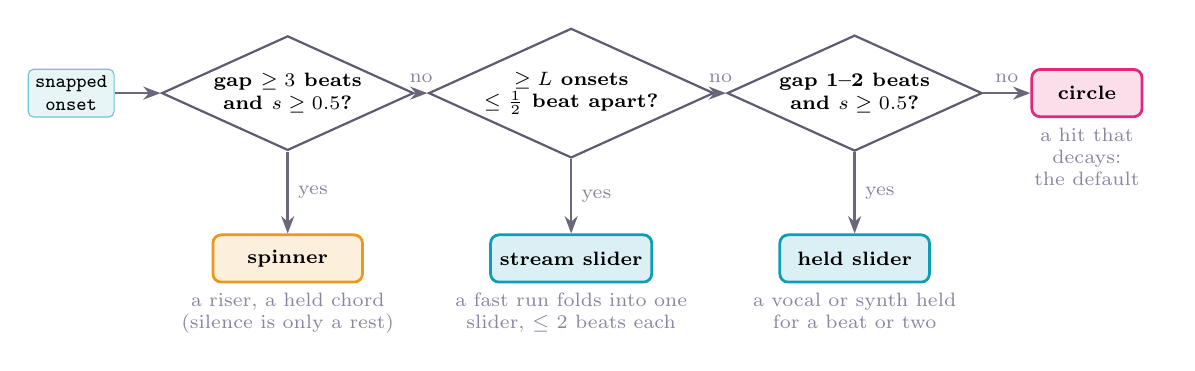
\begin{tikzpicture}[x=1cm,y=1cm,node distance=0.4cm]
    \node[data] (on) at (0,0) {snapped\\onset};
    \node[decision,alt=<2>{hot}{}] (d1) at (2.75,0) {gap $\ge3$ beats\\and $s\ge0.5$?};
    \node[decision,alt=<3>{hot}{}] (d2) at (6.35,0) {$\ge L$ onsets\\$\le\frac12$ beat apart?};
    \node[decision,alt=<4>{hot}{}] (d3) at (9.95,0) {gap 1--2 beats\\and $s\ge0.5$?};
    \node[outcome=amber] (sp) at (2.75,-2.1) {spinner};
    \node[outcome=teal] (st) at (6.35,-2.1) {stream slider};
    \node[outcome=teal] (hs) at (9.95,-2.1) {held slider};
    \node[outcome=magenta,minimum width=1.4cm] (ci) at (12.9,0) {circle};
    \draw[flow] (on) -- (d1);
    \draw[flow,alt=<3->{hotflow}{}] (d1) -- node[above,note] {no} (d2);
    \draw[flow,alt=<4->{hotflow}{}] (d2) -- node[above,note] {no} (d3);
    \draw[flow,alt=<5>{hotflow}{}] (d3) -- node[above,note] {no} (ci);
    \draw[flow,alt=<2>{hotflow}{}] (d1) -- node[right,note] {yes} (sp);
    \draw[flow,alt=<3>{hotflow}{}] (d2) -- node[right,note] {yes} (st);
    \draw[flow,alt=<4>{hotflow}{}] (d3) -- node[right,note] {yes} (hs);
    \node[note,text width=3cm,anchor=north] at (sp.south) {a riser, a held chord\\(silence is only a rest)};
    \node[note,text width=3.2cm,anchor=north] at (st.south) {a fast run folds into one slider, $\le$ 2 beats each};
    \node[note,text width=3cm,anchor=north] at (hs.south) {a vocal or synth held for a beat or two};
    \node[note,text width=1.8cm,anchor=north] at (ci.south) {a hit that decays: the default};
  \end{tikzpicture}
  \vspace{0.6em}

  {\small ``Clean'' gaps only: if a thinned-out onset sat inside the gap, the sound was re-struck,
  so it cannot be a hold. \ $L$ (stream length) rises with the tier: Easy folds every run,
  Expert keeps each note as a circle.}
\end{frame}

\begin{frame}{Placement: distance snap}
  \begin{columns}[c]
    \begin{column}{0.5\textwidth}
      Mappers place the next object a fixed number of \textbf{circle diameters} per beat of
      elapsed time -- the editor's \emph{distance snap}. We do the same:
      \[ d=D\cdot\sigma\cdot\Delta b,\qquad D=2\,(54.4-4.48\,\mathrm{CS}) \]
      \vspace{-1.2em}
      \begin{itemize}\small
        \item $\sigma$: diameters per beat (0.85 Easy $\rightarrow$ 2.10 Expert)
        \item spacing is \textbf{linear in time}: a 1/1 gap reads as twice a 1/2 gap
        \item spacing tracks circle size, so patterns read the same at any CS
      \end{itemize}
    \end{column}
    \begin{column}{0.48\textwidth}
      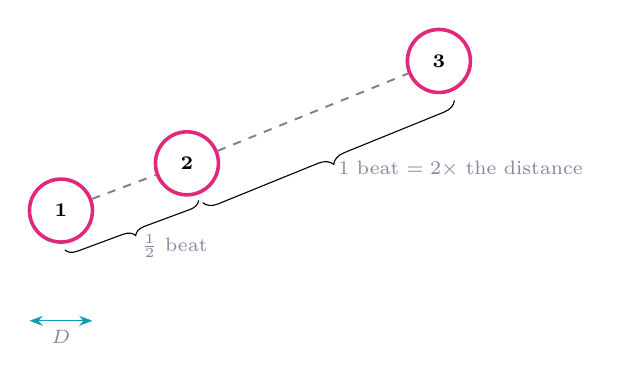
\begin{tikzpicture}[x=1cm,y=1cm]
        \node[pfcircle,minimum size=0.8cm] (a) at (0,0) {1};
        \node[pfcircle,minimum size=0.8cm,visible on=<2->] (b) at (1.6,0.6) {2};
        \node[pfcircle,minimum size=0.8cm,visible on=<3->] (c) at (4.8,1.9) {3};
        \draw[pfpath,visible on=<2->] (a) -- (b);
        \draw[pfpath,visible on=<3->] (b) -- (c);
        \draw[decorate,decoration={brace,amplitude=4pt,mirror},visible on=<2->] (0.05,-0.5) -- (1.75,0.13)
          node[midway,below right,note] {$\tfrac12$ beat};
        \draw[decorate,decoration={brace,amplitude=5pt,mirror},visible on=<3->] (1.8,0.1) -- (5.0,1.4)
          node[midway,below right,note] {1 beat $=2\times$ the distance};
        \draw[{Stealth}-{Stealth},teal,visible on=<4->] (-0.4,-1.4) -- node[below,note] {$D$} (0.4,-1.4);
      \end{tikzpicture}
    \end{column}
  \end{columns}
\end{frame}

\begin{frame}{Placement: flow and readability}
  \begin{columns}[c]
    \begin{column}{0.5\textwidth}
      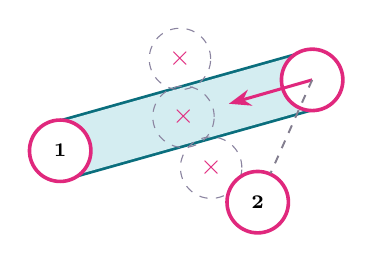
\begin{tikzpicture}[x=1cm,y=1cm]
        % the slider just played, and the cursor at its end
        \draw[teal!70!black,line width=22pt,line cap=round] (-1.4,-0.4) -- (1.8,0.5);
        \draw[teal!18,line width=20pt,line cap=round] (-1.4,-0.4) -- (1.8,0.5);
        \node[pfcircle,minimum size=0.78cm] at (-1.4,-0.4) {1};
        \node[pfcircle,minimum size=0.78cm] at (1.8,0.5) {};
        % the heading the flow asks for: a sharp turn back
        \draw[-{Stealth},line width=1.1pt,magenta] (1.8,0.5) -- ($(1.8,0.5)+(196:1.1)$);
        % candidates at 0, +25, -25, +50 degrees off the heading
        \foreach \a/\s in {0/2,-25/3,25/4}{
          \node[circle,draw=muted,dashed,minimum size=0.78cm,visible on=<\s->] at ($(1.8,0.5)+(196+\a:1.7)$) {};
          \node[font=\bfseries,text=magenta,visible on=<\s->] at ($(1.8,0.5)+(196+\a:1.7)$) {$\times$};
        }
        \node[pfcircle,minimum size=0.78cm,visible on=<5->] at ($(1.8,0.5)+(246:1.7)$) {2};
        \draw[pfpath,visible on=<5->] (1.8,0.5) -- ($(1.8,0.5)+(246:1.3)$);
      \end{tikzpicture}
      \par\centering\color{muted}\scriptsize \only<1>{magenta: the heading the flow asks for -- a sharp turn back}\only<2-4>{candidate hits the slider body: rotate and retry}\only<5->{first candidate that passes every rule}\par
    \end{column}
    \begin{column}{0.48\textwidth}\small
      A virtual cursor walks the objects in time order:
      \begin{enumerate}
        \item \textbf{Flow}: the heading turns only a little across short gaps (streams arc
              smoothly), freely across long ones (jumps). Max turn 40\textdegree\ Easy
              $\rightarrow$ 130\textdegree\ Expert.
        \item \textbf{Never bury}: $\ge0.75\,D$ from the previous object ($0.65\,D$ in a stream).
        \item \textbf{Stay off slider bodies}: clear the \emph{drawn curve}, not just its ends.
      \end{enumerate}
      \uncover<2->{Candidates are tried at $0^\circ,\pm25^\circ,\pm50^\circ,\dots$ off the
      heading; near a wall the heading is nudged back to the centre.}
    \end{column}
  \end{columns}
\end{frame}

\begin{frame}{The result on the playfield}
  \begin{columns}[c]
    \begin{column}{0.55\textwidth}
      \centering
      \begin{tikzpicture}[x=\statPFScale cm,y=-\statPFScale cm]
        \draw[void!40,fill=void!3,rounded corners=2pt] (0,0) rectangle (512,384);
        \draw[void!15,dashed] (40,40) rectangle (472,344);
        \node[note,anchor=south west] at (0,0) {$512\times384$ osu!px};
        \input{data/playfield.tex}
      \end{tikzpicture}
    \end{column}
    \begin{column}{0.43\textwidth}\small
      \textbf{\statTier}, \statPFCount\ consecutive objects of \SongFile\ in play order,
      drawn at true scale (circle radius \statPFRadius\,px).\\[0.6em]
      \begin{itemize}
        \item dashed line: the cursor path the player's hand takes
        \item the slider's next object leaves from its \emph{end}, off to one side of the body
        \item a stream keeps curving the same way
      \end{itemize}
      \medskip
      {\color{muted}Only objects within one approach time ($\sim$1\,s) are on screen together.}
    \end{column}
  \end{columns}
\end{frame}

\begin{frame}{Slider shapes and timing}
  \begin{columns}[T]
    \begin{column}{0.55\textwidth}
      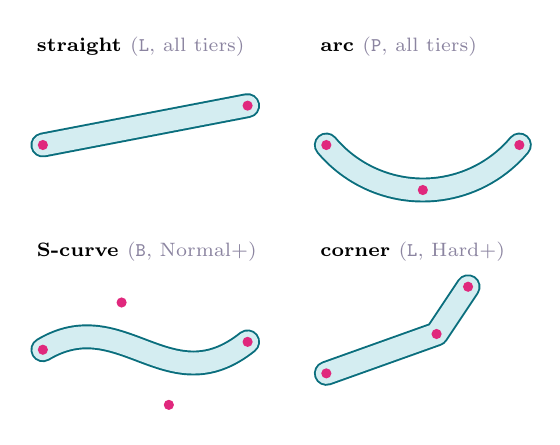
\begin{tikzpicture}[x=1cm,y=1cm,sl/.style={teal!70!black,line width=9pt,line cap=round},
                          sli/.style={teal!18,line width=7.6pt,line cap=round},
                          anc/.style={circle,fill=magenta,inner sep=1.3pt}]
        \foreach \s/\x/\name/\tier/\letter in {1/0/straight/all tiers/L,2/3.6/arc/all tiers/P,3/0/S-curve/Normal+/B,4/3.6/corner/Hard+/L}{
          \node[visible on=<\s->,font=\scriptsize\bfseries,anchor=west] at (\x,{\s>2 ? -1.35 : 1.25}) {\name\ {\color{muted}\normalfont(\texttt{\letter}, \tier)}};
        }
        \begin{scope}[visible on=<1->]
          \draw[sl] (0.2,0) -- (2.8,0.5); \draw[sli] (0.2,0) -- (2.8,0.5);
          \node[anc] at (0.2,0) {}; \node[anc] at (2.8,0.5) {};
        \end{scope}
        \begin{scope}[visible on=<2->]
          \draw[sl] (3.8,0) arc[start angle=220,end angle=320,radius=1.6];
          \draw[sli] (3.8,0) arc[start angle=220,end angle=320,radius=1.6];
          \node[anc] at (3.8,0) {}; \node[anc] at ($(3.8,0)+(220:-1.6)+(270:1.6)$) {};
          \node[anc] at ($(3.8,0)+(220:-1.6)+(320:1.6)$) {};
        \end{scope}
        \begin{scope}[visible on=<3->]
          \draw[sl] (0.2,-2.6) .. controls (1.2,-2.0) and (1.8,-3.3) .. (2.8,-2.5);
          \draw[sli] (0.2,-2.6) .. controls (1.2,-2.0) and (1.8,-3.3) .. (2.8,-2.5);
          \foreach \p in {(0.2,-2.6),(1.2,-2.0),(1.8,-3.3),(2.8,-2.5)} \node[anc] at \p {};
        \end{scope}
        \begin{scope}[visible on=<4->]
          \draw[sl,line join=round] (3.8,-2.9) -- (5.2,-2.4) -- (5.6,-1.8);
          \draw[sli,line join=round] (3.8,-2.9) -- (5.2,-2.4) -- (5.6,-1.8);
          \foreach \p in {(3.8,-2.9),(5.2,-2.4),(5.6,-1.8)} \node[anc] at \p {};
        \end{scope}
      \end{tikzpicture}
    \end{column}
    \begin{column}{0.43\textwidth}\small
      \textbf{Timing is fixed first}, shape second. The game derives a slider's duration
      from its length:
      \[ \text{beats}=\frac{L\cdot\text{slides}}{100\cdot\mathrm{SM}\cdot\mathrm{SV}} \]
      so $L$ is solved for the beats Step 4 wanted.\\[0.5em]
      \uncover<5->{Every curve must pass: no kink at the head, stays on the playfield,
      never closer to recent objects than its own head, leaves room to exit. Otherwise the
      straight slider is used.\\[0.4em]
      {\color{muted}Measured on six songs: buried objects 69 $\rightarrow$ 33.}}
    \end{column}
  \end{columns}
\end{frame}

% ======================================================================
\sectionframe{5}{Difficulty scaling}{One analysis, five maps}
\section{5 \;Difficulty}

\begin{frame}{Five parameter sets over one analysis}
  \begin{columns}[T]
    \begin{column}{0.54\textwidth}\scriptsize
      \begin{tabular}{@{}lccc@{}}
        \toprule
        knob & Easy & Hard & Expert\\
        \midrule
        $\lambda$ / $\delta$ & 2.2 / .08 & 1.5 / .05 & 1.1 / .03\\
        snap grid & 1/1 & 1/4 & 1/4\\
        min spacing (beats) & 2.0 & 0.5 & 0.25\\
        stream length $L$ & 4 & 6 & 999\\
        distance $\sigma$ & 0.85 & 1.3 & 2.10\\
        max turn & 40\textdegree & 75\textdegree & 130\textdegree\\
        AR / OD / CS & 4 / 3 / 3.2 & 7.5 / 6 / 4 & 9.3 / 8.5 / 4.2\\
        \bottomrule
      \end{tabular}\\[0.6em]
      {\color{muted}\scriptsize full table: \texttt{configs/difficulty\_presets.yaml}}\\[0.6em]
      \uncover<2->{The \textbf{DSP} knobs ($\lambda$, $\delta$) decide how many onsets
      exist; the \textbf{musical} knobs decide how many survive and how they move.}
    \end{column}
    \begin{column}{0.44\textwidth}
      \begin{tikzpicture}
        \begin{axis}[width=\linewidth,height=5.3cm,ybar,bar width=6pt,axis lines=left,ymin=0,
                     symbolic x coords={Easy,Normal,Hard,Insane,Expert},xtick=data,
                     ylabel={count},legend style={font=\tiny,at={(0.02,0.98)},anchor=north west,draw=none,fill=none},
                     nodes near coords,every node near coord/.append style={font=\tiny,rotate=90,anchor=west}]
          \addplot[fill=teal,draw=none] table[col sep=comma,x=tier,y=slots]{data/tiers.csv};
          \addlegendentry{rhythm slots}
          \only<2->{\addplot[fill=magenta,draw=none] table[col sep=comma,x=tier,y=objects]{data/tiers.csv};
                    \addlegendentry{objects}}
        \end{axis}
      \end{tikzpicture}
      \par\centering\color{muted}\scriptsize \SongFile, all five tiers\par
    \end{column}
  \end{columns}
\end{frame}

% ======================================================================
\sectionframe{6}{Export}{A file the real game accepts}
\section{6 \;Export}

\begin{frame}[fragile]{Rendering \texttt{osu file format v14}}
  \begin{columns}[T]
    \begin{column}{0.56\textwidth}
      \fvset{fontsize=\tiny,frame=single,rulecolor=\color{void!30},framesep=2mm}
      \VerbatimInput{data/osu_excerpt.txt}
    \end{column}
    \begin{column}{0.42\textwidth}\small
      \begin{itemize}
        \item \texttt{[Difficulty]}: the tier's preset
        \item<2-> \texttt{[TimingPoints]}: \emph{one} red line -- offset \statOffset\,ms,
              beat \statBeatMs\,ms (Step 3)
        \item<3-> \texttt{[HitObjects]}: one record per object\\
              {\scriptsize\texttt{x,y,time,type,\dots}; type bits 1 circle, 2 slider, 8 spinner, +4 new combo}
        \item<4-> a slider: curve letter + anchors, slides, length
              $\;\Rightarrow\; \frac{140\cdot1}{100\cdot1.4}=1$ beat
      \end{itemize}
      \uncover<5->{\medskip
      Audio + five \texttt{.osu} files, zipped $\rightarrow$ \texttt{Artist - Song.osz}.\\
      osu!(lazer) refuses malformed files, so a clean import \emph{is} the
      end-to-end test.}
    \end{column}
  \end{columns}
\end{frame}

\begin{frame}{Step 7: keeping what the DSP saw}
  \begin{columns}[c]
    \begin{column}{0.55\textwidth}
      The \texttt{.osu} format stores \emph{where} and \emph{when}, never \emph{why}.
      An extra export keeps the evidence:
      \begin{itemize}
        \item every onset with its \textbf{strength} and \textbf{dominant band}
        \item the beat grid, BPM and confidence
        \item each object's \textbf{snap} (1/1, 1/2, 1/4) and source onset
        \item the mel spectrogram as an image (max-pooled, so single-frame attacks survive)
      \end{itemize}
      \medskip
      {\color{muted}This is what the app visualises -- shown in the demo.}
    \end{column}
    \begin{column}{0.42\textwidth}
      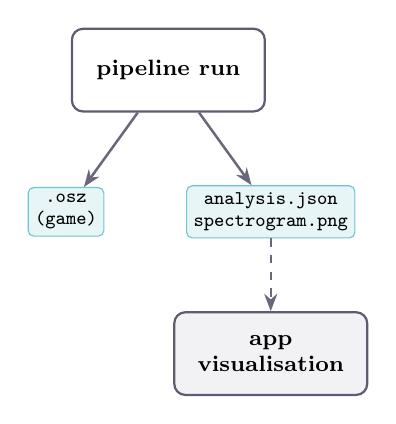
\begin{tikzpicture}[x=1cm,y=1cm]
        \node[stage] (p) at (0,0) {pipeline run};
        \node[data] (o) at (-1.3,-1.8) {.osz\\(game)};
        \node[data] (a) at (1.3,-1.8) {analysis.json\\spectrogram.png};
        \node[stage,fill=void!6] (v) at (1.3,-3.6) {app\\visualisation};
        \draw[flow] (p) -- (o); \draw[flow] (p) -- (a); \draw[flow,dashed] (a) -- (v);
      \end{tikzpicture}
    \end{column}
  \end{columns}
\end{frame}

% ======================================================================
\section{Validation}
\begin{frame}{How do you test a detector with no ground truth?}
  \begin{columns}[T]
    \begin{column}{0.32\textwidth}
      \begin{block}{1 \ Synthetic signals}\small
        Click tracks at a known BPM; held tones; 1/4 bursts.
        Exact expectations: every click found, tempo recovered, the held tone becomes a
        spinner, the burst folds into a slider.
      \end{block}
    \end{column}
    \begin{column}{0.32\textwidth}
      \begin{block}{2 \ Listening tests}\small
        \textbf{Sonification}: mix a click at every onset, or a metronome at every beat,
        and listen. Drift and double triggers are obvious by ear -- the standard check in
        music information retrieval.
      \end{block}
    \end{column}
    \begin{column}{0.32\textwidth}
      \begin{block}{3 \ Play-testing}\small
        Import into osu!(lazer) and play. Real feedback (overlaps, circles hidden under
        slider bodies) became automated placement tests.
      \end{block}
    \end{column}
  \end{columns}
  \bigskip
  \begin{center}
    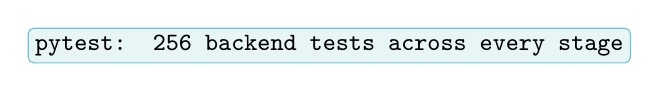
\begin{tikzpicture}
      \node[data,font=\small\ttfamily] {pytest: 256 backend tests across every stage};
    \end{tikzpicture}
  \end{center}
\end{frame}

% ======================================================================
\section{Summary}
\begin{frame}{Summary}
  \centering
  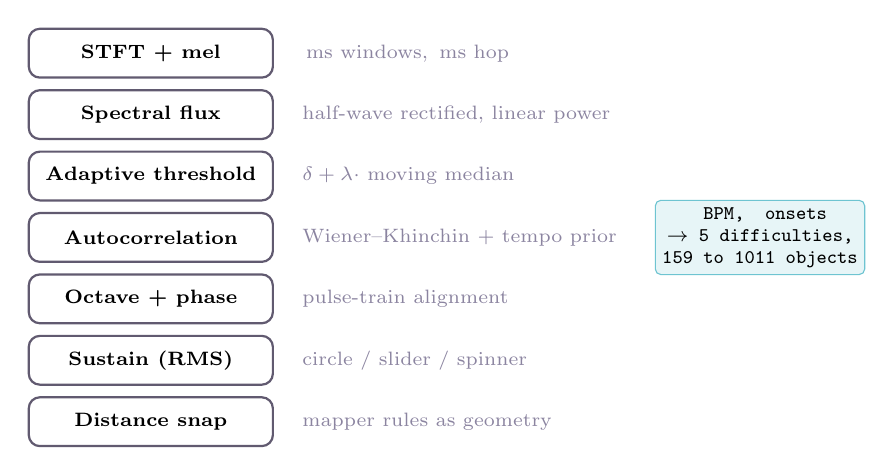
\begin{tikzpicture}[x=1cm,y=1cm]
    \foreach \i/\n/\d [count=\c] in {
      0/{STFT + mel}/{\statWinMs\,ms windows, \statHopMs\,ms hop},
      1/{Spectral flux}/{half-wave rectified, linear power},
      2/{Adaptive threshold}/{$\delta+\lambda\cdot$ moving median},
      3/{Autocorrelation}/{Wiener--Khinchin + tempo prior},
      4/{Octave + phase}/{pulse-train alignment},
      5/{Sustain (RMS)}/{circle / slider / spinner},
      6/{Distance snap}/{mapper rules as geometry}}{
      \node[stage,minimum width=3.1cm,minimum height=0.62cm,font=\scriptsize\bfseries,
            visible on=<\c->,alt=<\c>{hot}{}] (s\i) at (0,-0.78*\i) {\n};
      \node[note,anchor=west,visible on=<\c->] at (1.8,-0.78*\i) {\d};
    }
    \node[data,anchor=west,visible on=<8->] at (6.4,-2.34) {\statBPM\ BPM, \statOnsetsTotal\ onsets\\$\rightarrow$ 5 difficulties,\\159 to 1011 objects};
  \end{tikzpicture}
  \vspace{0.4em}

  \uncover<8->{\small\textbf{Limits \& next steps:} variable tempo, a real star-rating model,
  hitsounds, per-section slider velocity.}
\end{frame}

\begin{frame}[plain]
  \begin{tikzpicture}[remember picture,overlay]
    \fill[void] (current page.south west) rectangle (current page.north east);
    \node[text=white,font=\fontsize{30}{34}\selectfont\bfseries] at (current page.center) {Demo};
    \node[text=white!60!magenta,font=\large] at ($(current page.center)+(0,-1)$) {the app, end to end};
  \end{tikzpicture}
\end{frame}

\end{document}
